\documentclass{beamer}
\usepackage{amsmath}
\usepackage{hyperref}
\usepackage{listings}
\usepackage{xcolor}
\hypersetup{colorlinks=true, citecolor=blue, filecolor=blue, linkcolor=blue, urlcolor=blue}
\definecolor{codegreen}{rgb}{0,0.6,0}
\definecolor{codegray}{rgb}{0.5,0.5,0.5}
\definecolor{codepurple}{rgb}{0.58,0,0.82}
\definecolor{backcolour}{rgb}{0.95,0.95,0.92}
 
\lstdefinestyle{mystyle}{
    backgroundcolor=\color{backcolour},   
    commentstyle=\color{codegreen},
    keywordstyle=\color{magenta},
    numberstyle=\tiny\color{codegray},
    stringstyle=\color{codepurple},
    basicstyle=\ttfamily\footnotesize,
    breakatwhitespace=false,         
    breaklines=true,                 
    captionpos=b,                    
    keepspaces=true,                 
    %numbers=left,                    
    numbersep=5pt,                  
    showspaces=false,                
    showstringspaces=false,
    showtabs=false,                  
    tabsize=2
}
 
\lstset{style=mystyle}

\mode<presentation> {

% The Beamer class comes with a number of default slide themes
% which change the colors and layouts of slides. Below this is a list
% of all the themes, uncomment each in turn to see what they look like.

%\usetheme{default}
\usetheme{AnnArbor}
%\usetheme{Antibes}
%\usetheme{Bergen}
%\usetheme{Berkeley}
%\usetheme{Berlin}
%\usetheme{Boadilla}
%\usetheme{CambridgeUS}
%\usetheme{Copenhagen}
%\usetheme{Darmstadt}
%\usetheme{Dresden}
%\usetheme{Frankfurt}
%\usetheme{Goettingen}
%\usetheme{Hannover}
%\usetheme{Ilmenau}
%\usetheme{JuanLesPins}
%\usetheme{Luebeck}
%\usetheme{Madrid}
%\usetheme{Malmoe}
%\usetheme{Marburg}
%\usetheme{Montpellier}
%\usetheme{PaloAlto}
%\usetheme{Pittsburgh}
%\usetheme{Rochester}
%\usetheme{Singapore}
%\usetheme{Szeged}
%\usetheme{Warsaw}

% As well as themes, the Beamer class has a number of color themes
% for any slide theme. Uncomment each of these in turn to see how it
% changes the colors of your current slide theme.

%\usecolortheme{albatross}
%\usecolortheme{beaver}
%\usecolortheme{beetle}
%\usecolortheme{crane}
%\usecolortheme{dolphin}
%\usecolortheme{dove}
%\usecolortheme{fly}
%\usecolortheme{lily}
%\usecolortheme{orchid}
%\usecolortheme{rose}
%\usecolortheme{seagull}
%\usecolortheme{seahorse}
%\usecolortheme{whale}
%\usecolortheme{wolverine}

%\setbeamertemplate{footline} % To remove the footer line in all slides uncomment this line
\setbeamertemplate{footline}[page number] % To replace the footer line in all slides with a simple slide count uncomment this line

\setbeamertemplate{navigation symbols}{} % To remove the navigation symbols from the bottom of all slides uncomment this line
}

\usepackage{graphicx} % Allows including images
\usepackage{booktabs} % Allows the use of \toprule, \midrule and \bottomrule in tables
%\usepackage {tikz}
\usepackage{tkz-graph}
\GraphInit[vstyle = Shade]
\tikzset{
  LabelStyle/.style = { rectangle, rounded corners, draw,
                        minimum width = 2em, fill = yellow!50,
                        text = red, font = \bfseries },
  VertexStyle/.append style = { inner sep=5pt,
                                font = \normalsize\bfseries},
  EdgeStyle/.append style = {->, bend left} }
\usetikzlibrary {positioning}
%\usepackage {xcolor}
\definecolor {processblue}{cmyk}{0.96,0,0,0}
%----------------------------------------------------------------------------------------
%	TITLE PAGE
%----------------------------------------------------------------------------------------

\title[Surrogate Optimization]{Numerical Optimization 16: Surrogate Optimization} %

\author{Qiang Zhu} % Your name
\institute[University of Nevada Las Vegas] % Your institution as it will appear on the bottom of every slide, may be shorthand to save space
{
University of Nevada Las Vegas\\ % Your institution for the title page
\medskip
}
\date{\today} % Date, can be changed to a custom date

\begin{document}

\begin{frame}
\titlepage % Print the title page as the first slide
\end{frame}

\begin{frame}
\frametitle{Overview} % Table of contents slide, comment this block out to remove it
\tableofcontents % Throughout your presentation, if you choose to use \section{} and \subsection{} commands, these will automatically be printed on this slide as an overview of your presentation
\end{frame}

%----------------------------------------------------------------------------------------
%	PRESENTATION SLIDES
%----------------------------------------------------------------------------------------

%------------------------------------------------

\section{Prediction-Based Exploration}
\begin{frame}{Prediction-Based Exploration}
Gaussian process probes the probability distributions over the true objective function. These distributions can be used to guide an optimization process toward better design points. In prediction-based exploration, we select the minimizer of the surrogate function. If we use a Gaussian process surrogate model, prediction-based optimization has us select the minimizer of the mean function
\begin{equation*}
    \boldsymbol{x}^{m+1} = \underset{\boldsymbol{x}\in \chi}{\arg\min}~~ \hat{\boldsymbol{\mu}}(\boldsymbol{x})
\end{equation*}

where $\hat{\boldsymbol{\mu}}(\boldsymbol{x})$ is the predicted mean of a Gaussian process at a design point $x$ based on the previous m design points. 

Prediction-based optimization does not take uncertainty into account, and new samples can be generated very close to existing samples, which is a waste of time.
\end{frame}

\section{Error-Based Exploration}
\begin{frame}{Error-Based Exploration}
Error-based exploration seeks to increase confidence in the true function. A Gaussian process can tell us both the mean and standard deviation at every point. The next sample point is:
\begin{equation*}
    \boldsymbol{x}^{m+1} = \underset{\boldsymbol{x}\in \chi}{\arg\max}~~ \hat{\boldsymbol{\sigma}}(\boldsymbol{x})
\end{equation*}
where $\hat{\boldsymbol{\sigma}}(\boldsymbol{x})$ is the predicted standard variance of a Gaussian process at a design point $x$ based on the previous m design points. 

\begin{figure}
\centering
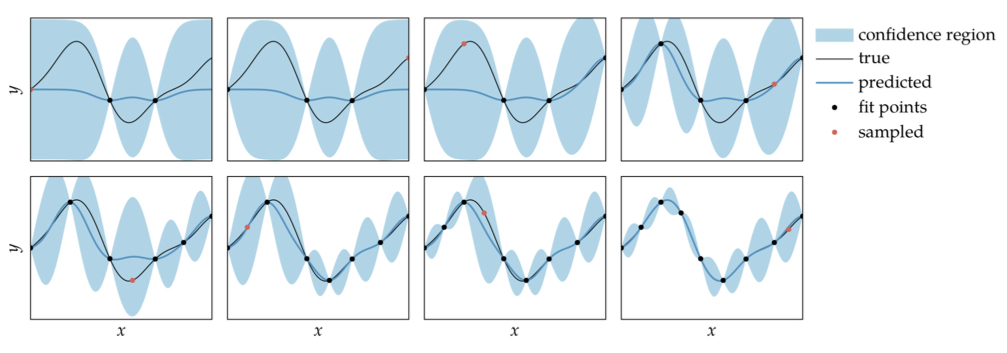
\includegraphics[width=120mm]{Figs/error-explore.jpeg}
\end{figure} 
\end{frame}


\section{Lower Confidence Bound Exploration}
\begin{frame}{Lower Confidence Bound Exploration}
The error-based exploration may sample the regions that are unpromising. Lower confidence bound exploration trades off between greedy minimization employed by prediction-based optimization and uncertainty reduction employed by error-based exploration with the following strategy,

\begin{gather*}
    LB(x) = \hat{\mu}(\boldsymbol{x})-\alpha \hat{\sigma}(\boldsymbol{x})
\end{gather*}
$\alpha \geq 0$ is to control the trade-off between exploration and exploitation. 
\begin{figure}
\centering
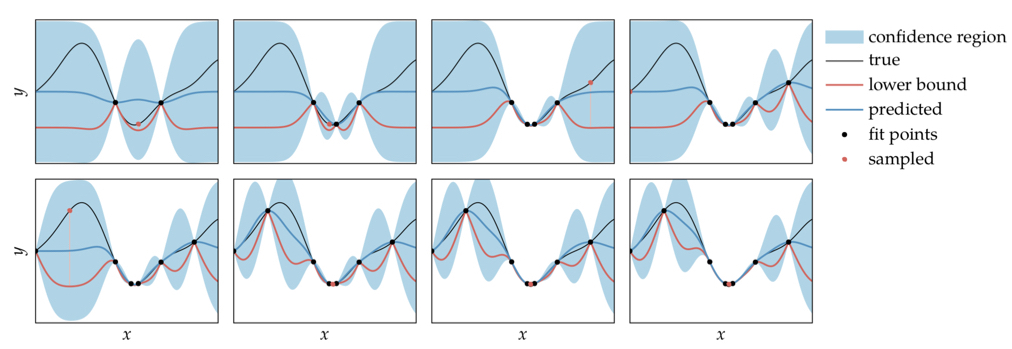
\includegraphics[width=120mm]{Figs/LB.jpeg}
\end{figure} 

\end{frame}

\section{Probability of Improvement Exploration}
\begin{frame}{Probability of Improvement Exploration}
We select the design point that maximizes the chance that the new point will be better than any other. The improvement for a function sampled at $x$ producing $y=f(x)$ is
\begin{equation*}
    I(y) = 
    \begin{cases}
    y_{\min} - y & \textrm{if~} y<y_{\min}\\
    0 & {\textrm{otherwise}}\\
    \end{cases}
\end{equation*}
The probability of improvement at points where $\hat{\sigma}>0$ is
\begin{equation*}
P(y<y_{\min}) = \int_0^{y_{\min}} \mathcal{N}(y| \hat{\mu}, \hat{\sigma})dy = \Phi(\frac{y_{\min}-\hat{\mu}}{\hat{\sigma}})
\end{equation*}

\begin{figure}
\centering
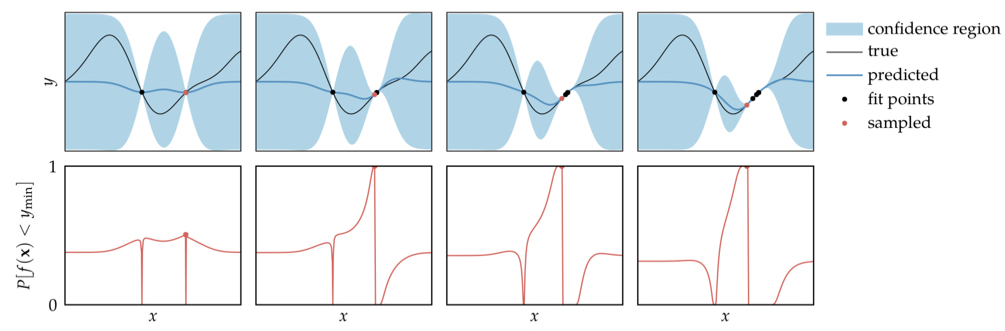
\includegraphics[width=100mm]{Figs/prob.jpeg}
\end{figure} 

\end{frame}

\section{Expected Improvement Exploration}
\begin{frame}{Expected Improvement Exploration}
We can also focus our exploration of points that maximize our expected improvement over the current best function value.
Through a substitution
\begin{equation*}
    z = \frac{y-\hat{\mu}}{\hat{\sigma}} ~~~~~~~~~~~ y`_{\min} = \frac{y_{\min} - \hat{\mu}}{\hat{\sigma}}
\end{equation*}
we can write the improvement as
\begin{equation*}
    I(y) = 
    \begin{cases}
    \hat{\sigma} (y`_{\min} -z) & {\textrm{if}~} z<y`_{\min} {\textrm{~and~}} \hat{\sigma} >0 \\
    0 & {\textrm{otherwise}}\\
    \end{cases}
\end{equation*}
where $\hat{\mu}$ and $\hat{\sigma}$ are the predicted mean and standard deviation.

We can calculate the expected improvement using Gaussian process:
\begin{equation*}
\begin{split}
    \mathbb{E}[I(y)] &= \hat{\sigma} \int_{-\infty}^{y`_{\min}}  \mathcal{N}(z|0,1)dz\\
    & = (y_{\min} - \hat{\mu}) P (y \leq y_{\min}) + \hat{\sigma} \mathcal{N}(y_{\min} | \hat{\mu}, \hat{\sigma}ˆ2)
\end{split}
\end{equation*}

\end{frame}

\begin{frame}{Expected Improvement Exploration}

\begin{figure}
\centering
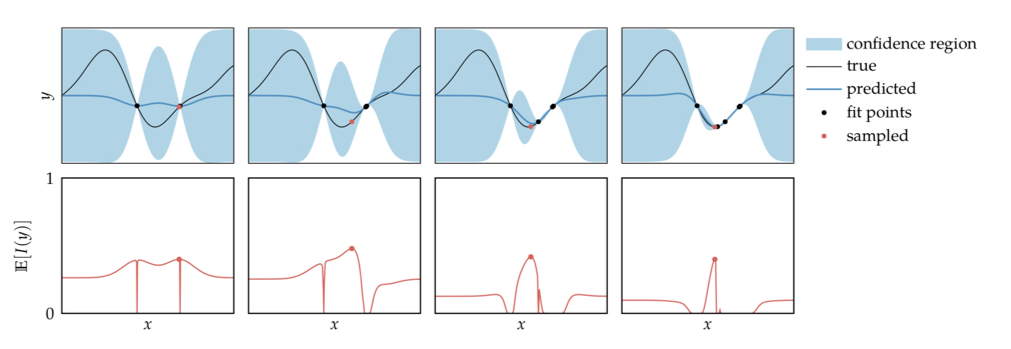
\includegraphics[width=125mm]{Figs/EI.jpeg}
\end{figure} 

\end{frame}

\section{Summary}
\begin{frame}{Summary}
    \begin{itemize}
        \item Gaussian processes can be used to guide the optimization process using a variety of strategies that use estimates of quantities such as the lower confidence bound, probability of improvement, and expected improvement.
        \item Some problems do not allow for the evaluation of unsafe designs, in which case we can use safe exploration strategies that rely on Gaussian processes.
    \end{itemize}
\end{frame}
\end{document}

